\subsection{插件登录 ECNU 及辅助登录}\label{subsec:plugin-login-ecnu}

插件许多功能需要调用 ECNU 提供的各种接口。
接口的调用依赖于 ECNU 各个系统的登录缓存(在项目内部保存为 \verb`LoginCache`)。
为了获取有效的登录缓存简化登录操作,
插件登录使用了 WebDriver 控制浏览器实现自动化或半自动化的辅助登录流程。

在插件登录时,会出现浏览器 ECNU 统一身份认证的界面,登录有两种方式。
\begin{itemize}
    \item 方法一:填写图\ref{fig:uia-login-form} 中的表单实现登录。
    \item 方法二:扫描图\ref{fig:uia-login-qrcode} 中的二维码实现登录。
\end{itemize}

\begin{table}[H]
    \centering
    \begin{tabular}{cc}
        \begin{minipage}[H]{0.5\textwidth}
            \centering
            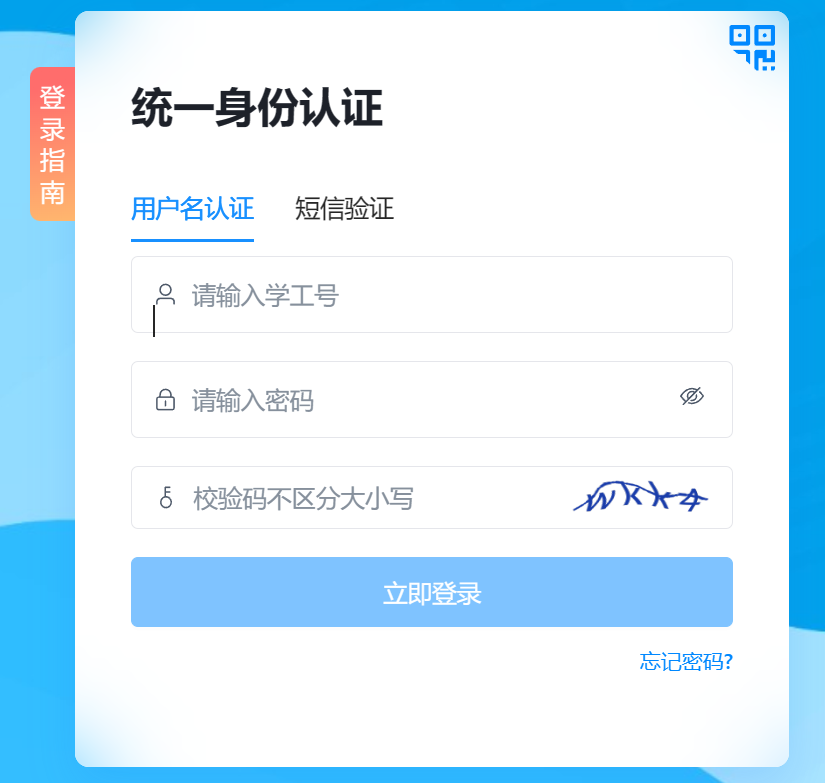
\includegraphics[width=0.8\textwidth]{img/uia_login_form}
            \captionof{figure}{ECNU UIA 登录界面(表单)}
            \label{fig:uia-login-form}
        \end{minipage} &
        \begin{minipage}[H]{0.5\textwidth}
            \centering
            
\includegraphics[width=0.8\textwidth]{img/uia_login_qrcode}
            \captionof{figure}{ECNU UIA 登录界面(二维码)}
            \label{fig:uia-login-qrcode}
        \end{minipage}
    \end{tabular}
\end{table}

\begin{rmr}[切换表单登录和二维码登录]
    \quad 表单登录:
    可以在项目根目录创建文件 \verb`login_info.toml`
    然后填写如下内容(替换尖括号以内的部分)。
    插件登录时会读取此文件中的学号密码,自动填写图\ref{fig:uia-login-form} 中的表单,实现全自动辅助登录。
    % @formatter:off
    \begin{verbatim}
stu_number = "<填写学号>"
password = "<填写数据库密码>" \end{verbatim}
    % @formatter:on

    \quad 二维码登录:
    删除 \verb`login_info.toml` 文件,
    此时插件辅助登录时会截取二维码图片并发送至邮箱提醒。
    可以使用微信扫描二维码或用微信打开邮件中的连接实现半自动登录。
\end{rmr}

\subsubsection{辅助登录具体实现}
% 以下内容均未更改,只是不小心格式化 fmt
\begin{enumerate}
    \item \textbf{初始化}:使用 Webdriver 启动浏览器并导航到 ECNU 座位筛选页面,该页面会重定向到统一认证登录页面。

    \item \textbf{基于二维码的登录}:
    \begin{itemize}
        \item 如果未找到凭证,则进行二维码登录:使用 CSS 选择器定位到二维码登录按钮;
        \item 之后提取二维码图片,解码以获取登录 URL,并将图片保存为临时文件;
        \item 使用回调函数(\texttt{qrcode\_callback})将二维码发送给用户(例如,通过邮件或微信)。
        \item 监控登录状态,处理二维码过期后的刷新。
    \end{itemize}

    \item \textbf{缓存提取}:
    \begin{itemize}
        \item 登录成功后,调用一系列 \texttt{cache\_grabbers} 函数提取必要的缓存数据。
        \item 将这些缓存存储在 \texttt{LoginCache} 实例中,以供其他组件或插件使用。
    \end{itemize}
\end{enumerate}

\begin{note}
    以上代码可以进入 \texttt{src/uia/login.py} 文件中查看,其中,核心函数 \texttt{get\_login\_cache} 已提供了完整的注释信息。

    但是,我们获得的 \texttt{login\_cache} 是会失活而非永久的,这一点通过查阅华东师范大学开发者文档可以得知:

    \href{https://developer.ecnu.edu.cn/vitepress/data/architecture/authorization.html}{\underline{https://developer.ecnu.edu.cn/vitepress/data/architecture/authorization.html}}
\end{note}

\begin{figure}[H]
    \centering
    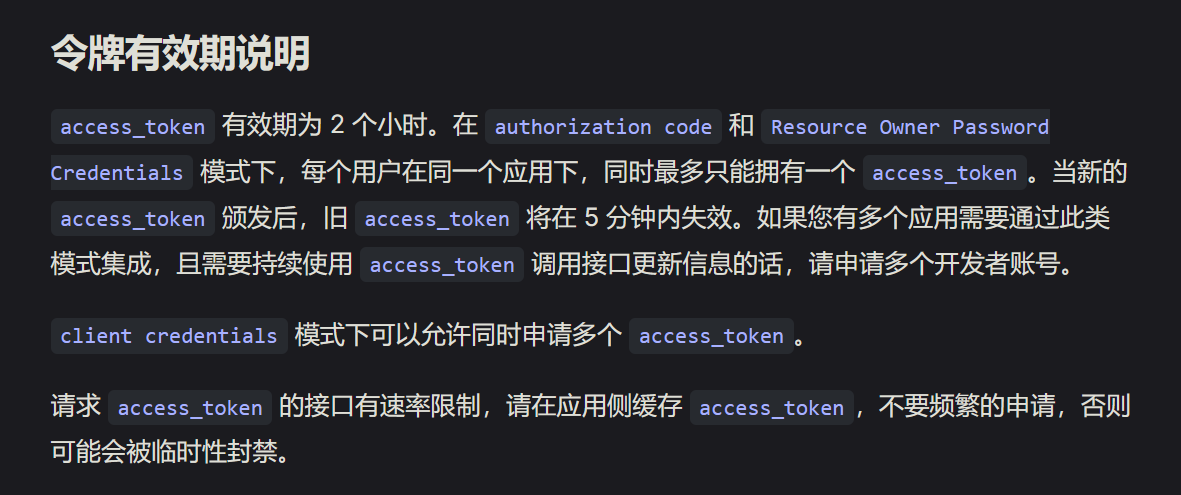
\includegraphics[width=0.5\textwidth]{img/open_platform.png}
    \caption{缓存过期时间}
    \label{fig:cache_expiration}
\end{figure}

\subsubsection{通过 OCR 识别验证码登录}

后来意识到,这样需要手动点击链接来刷新缓存的方式,违背了我们全自动化、便捷的初心,于是我们决定攻破验证码的防线,便在 Github 上寻找到了一个较为优秀的项目:
(DDDDOCR):\href{https://github.com/sml2h3/ddddocr}{\underline{https://github.com/sml2h3/ddddocr}}。

我们使用一段 JavaScript 代码成功提取了验证码图片,它是通过 \texttt{<img>} 标签加载在网页中的:

\begin{lstlisting}[language=python]
    EXTRACT_CAPTCHA_IMG_JS = f"""
    let img = document.querySelector("{CAPTCHA_IMG_SELECTOR}");
    let canvas = document.createElement('canvas');
    let ctx = canvas.getContext('2d');

    # 使用 canvas 画布在前端绘制图片,之后保存到文件中供 OCR 识别
    canvas.width = img.width;
    canvas.height = img.height;
    ctx.drawImage(img, 0, 0, canvas.width, canvas.height);
    return canvas.toDataURL('image/png');
    """
\end{lstlisting}

有时 OCR 的结果不是四位有效的验证码,所以我们添加了一行代码增大了准确性:

\begin{lstlisting}[language=Python]
    if len(captcha) != 4:
        driver.refresh()
\end{lstlisting}

尝试使用后,它有将近 $\frac{1}{3}$ 识别的准确率。此后,便可以实现自动化登录,解放双手了。
较为幸运的是,华师并未设置验证码多次登录失败后禁止登录的逻辑,所以成功率较低的情况下也可以照常使用。

最终,我们获取的 \texttt{LoginCache} 置于项目根目录中的文件 \texttt{login-cache.pickle} 中,
其中最重要的字段为 \textbf{Bearer} 字段以及 \textbf{cookie} 字段,这是在 \textbf{OAuth 2.0} 框架下在 HTTP 请求头中的认证类型,携带访问令牌通过 \textbf{Bearer Token} 来实现无状态的认证。

\begin{figure}[H]
    \centering
    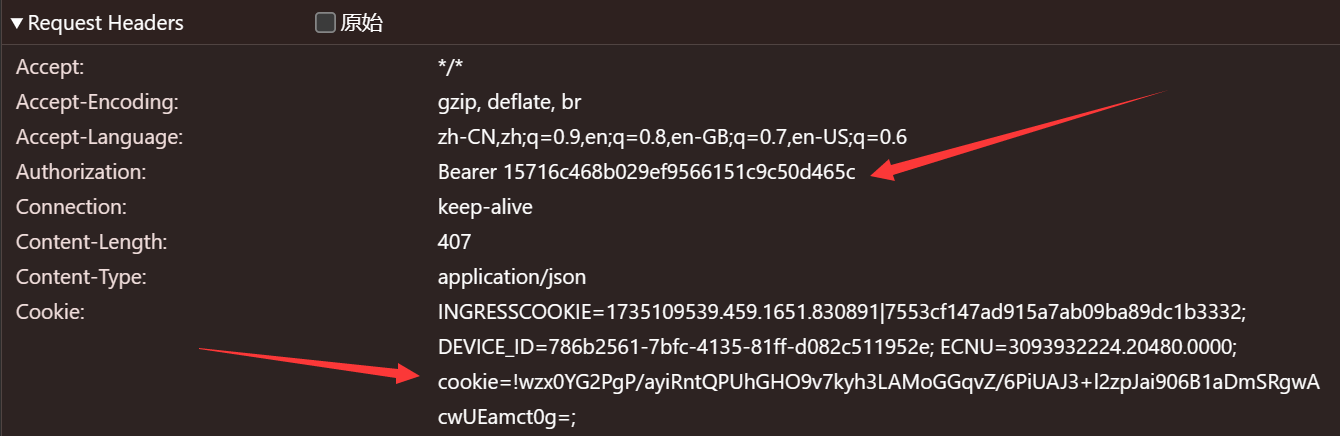
\includegraphics[width=0.66\textwidth]{img/main_cache.png}
    \caption{Main Cookie 及鉴权 Token}
    \label{fig:main_cache}
\end{figure}

华东师范大学开发者平台提供了一个 OAuth 2.0 的 Playground 调试平台,教师可进入以下网站进行在线调试:

\href{https://developer.ecnu.edu.cn/oauth2playground/}{\underline{https://developer.ecnu.edu.cn/oauth2playground/}}

\begin{figure}[H]
    \centering
    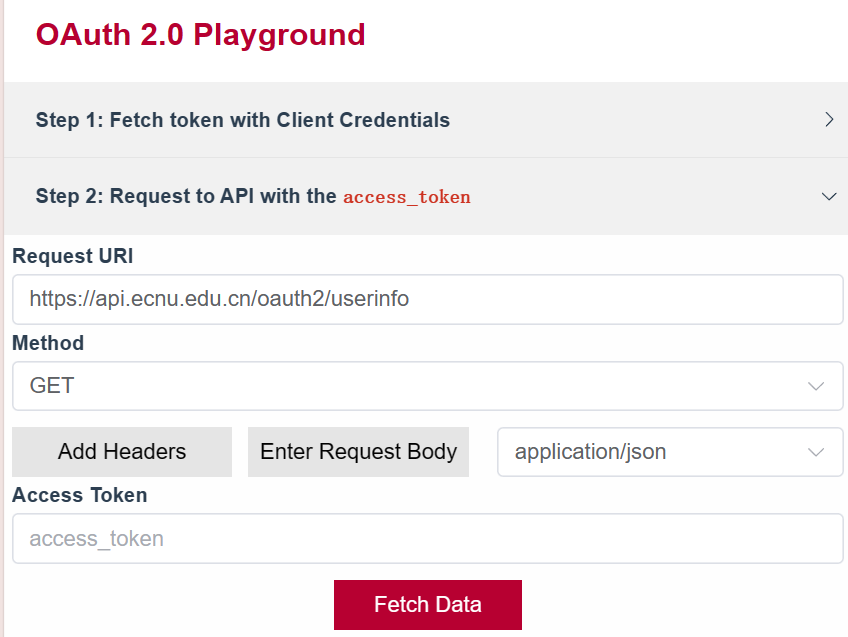
\includegraphics[width=0.42\textwidth]{img/OAuth2Playground.png}
    \caption{OAuth 2.0 Playground}
    \label{fig:oauth2_playground}
\end{figure}